\documentclass{article}
\usepackage[margin=1in]{geometry} 
\usepackage{amsmath}
\usepackage[T1]{fontenc}          % change font encoding to T1
\usepackage{lmodern}  %better for visual on screen
\usepackage{graphicx}
\usepackage{float}
\usepackage{enumitem}
\usepackage{mathtools}
\usepackage{booktabs}
\usepackage{dirtree}

\makeatletter
\renewcommand*\env@matrix[1][\arraystretch]{%
	\edef\arraystretch{#1}%
	\hskip -\arraycolsep
	\let\@ifnextchar\new@ifnextchar
	\array{*\c@MaxMatrixCols c}}
\makeatother

% Used for adding Matlab Algorithms
\RequirePackage{listings}
\RequirePackage[framed,numbered]{matlab-prettifier}

\DeclarePairedDelimiter\abs{\lvert}{\rvert}%

\begin{document}
\section{idw.m}
\lstinputlisting[
label      = {alg:lsr},
style      = Matlab-editor,
basicstyle = \mlttfamily,
firstline  = 1,
lastline   = 15,
firstnumber= 1
]{../idw.m}

\subsection{Motivation/Concept}
Inverse Distance Weighting(IDW) is a very common algorithm for interpolating sparse data.  IDW performs a weighted average on points within a certain radius based the equation:
\[
W = distance ^ {power}
\]
Or more formally
\begin{align*}
d_i &= \text{distance to point i} \\
p &= \text{idw power constant} \\
r &= \text{radius constant} \\
n &= \text{number of points within radius (r)} \\
Y &= \dfrac{\sum\limits_{i=1}^{n} y_id_i^p}{\sum\limits_{i=1}^{n} d_i^p}
\end{align*}

\subsection{Inputs/Outputs}
\lstinputlisting[
label      = {alg:lsr},
style      = Matlab-editor,
basicstyle = \mlttfamily,
firstline  = 17,
lastline   = 28,
firstnumber= 17
]{../idw.m}

\clearpage
\subsection{Examples \textit{exampleIdw.m}}
\subsubsection*{Example IDW Line}
This example demonstrates generation of a line using IDW with the default power of -2.
\lstinputlisting[
label      = {alg:lsr},
style      = Matlab-editor,
basicstyle = \mlttfamily,
firstline  = 2,
lastline   = 8,
firstnumber= 3
]{../exampleIdw.m}

\begin{figure}[H]
	\centering
	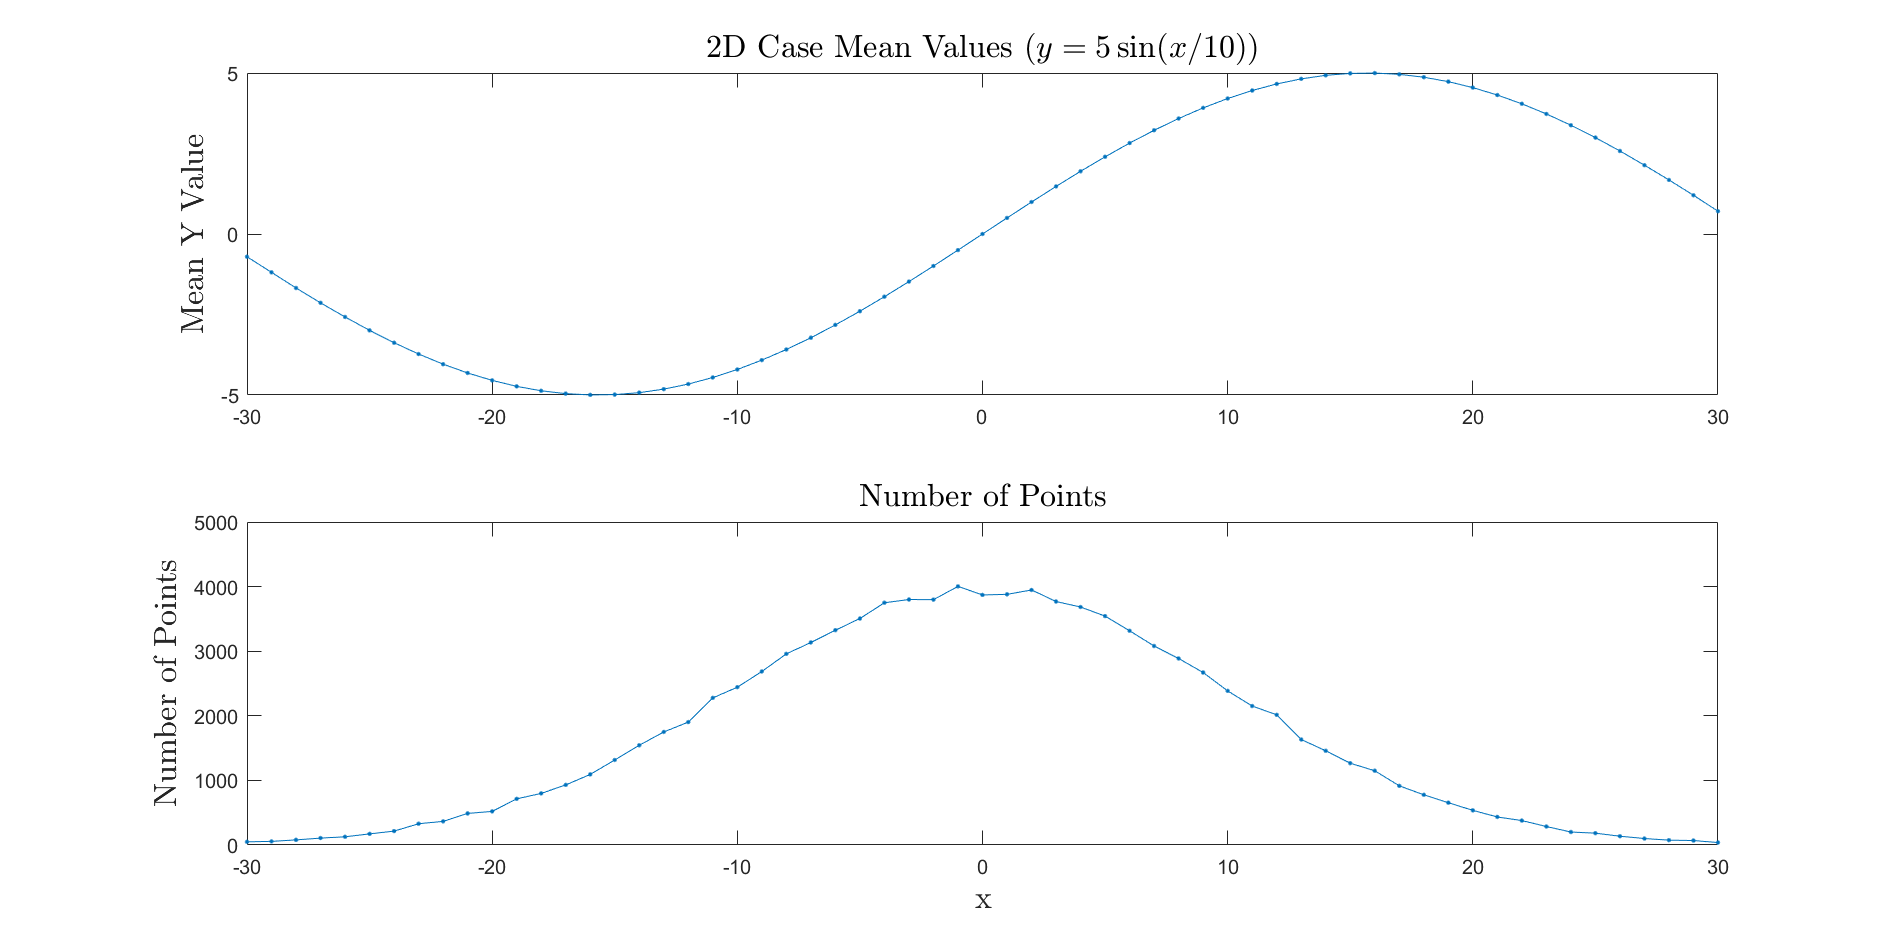
\includegraphics[width = \linewidth]{1d}
\end{figure}
\clearpage

\subsubsection*{Example IDW 2D}
This example demonstrates generation of a plane grid using IDW with the default power of -2.
\lstinputlisting[
label      = {alg:lsr},
style      = Matlab-editor,
basicstyle = \mlttfamily,
firstline  = 23,
lastline   = 31,
firstnumber= 23
]{../exampleIdw.m}

\begin{figure}[H]
	\centering
	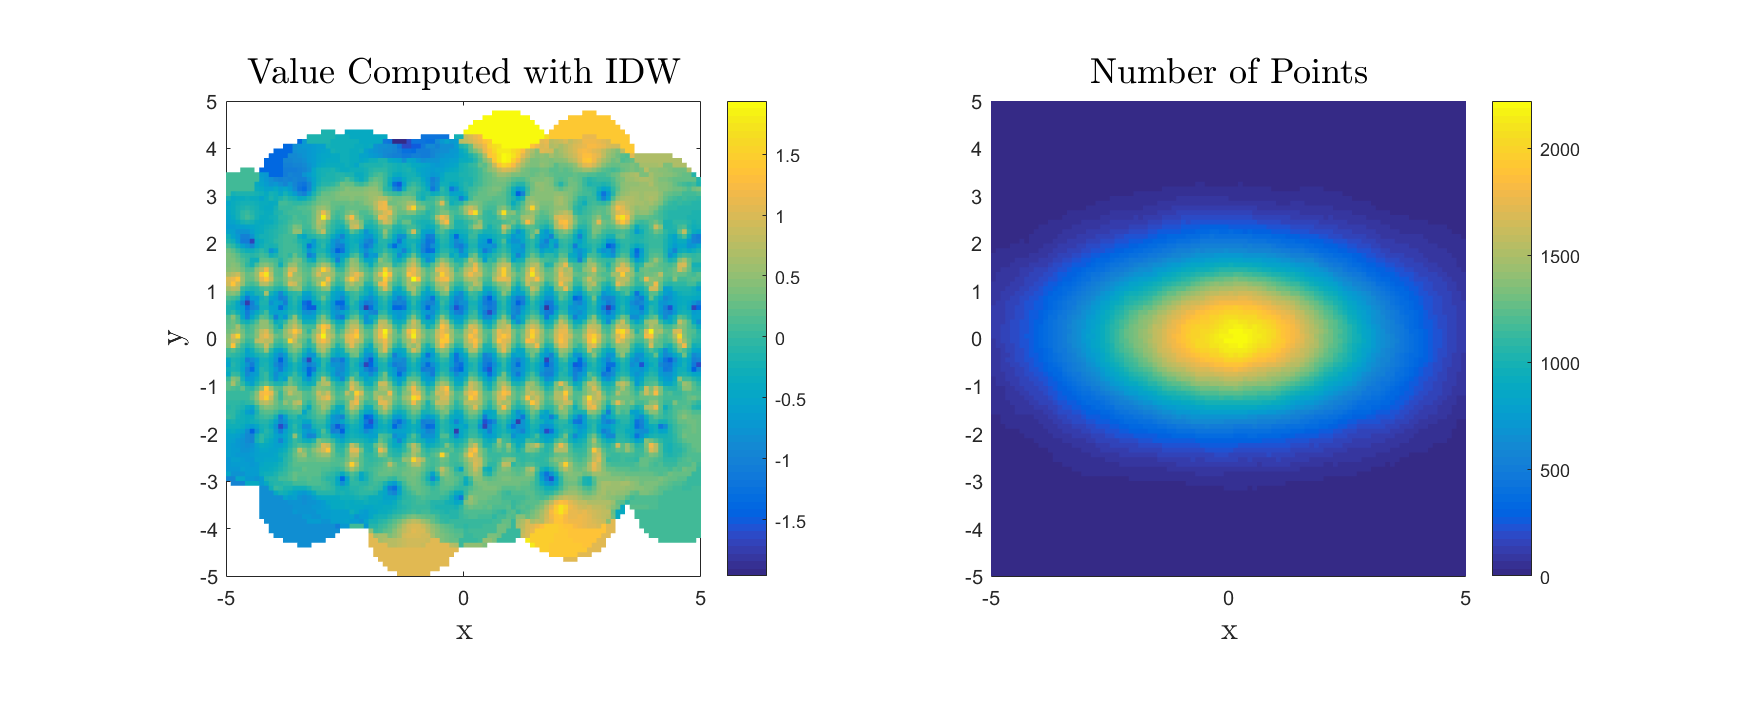
\includegraphics[width = \linewidth]{example3d}
\end{figure}
\clearpage

\subsubsection*{Example IDW Plane (Power = -1)}
This example demonstrates generation of a plane grid using IDW with a power of -1.
\lstinputlisting[
label      = {alg:lsr},
style      = Matlab-editor,
basicstyle = \mlttfamily,
firstline  = 52,
lastline   = 60,
firstnumber= 52
]{../exampleIdw.m}

\begin{figure}[H]
	\centering
	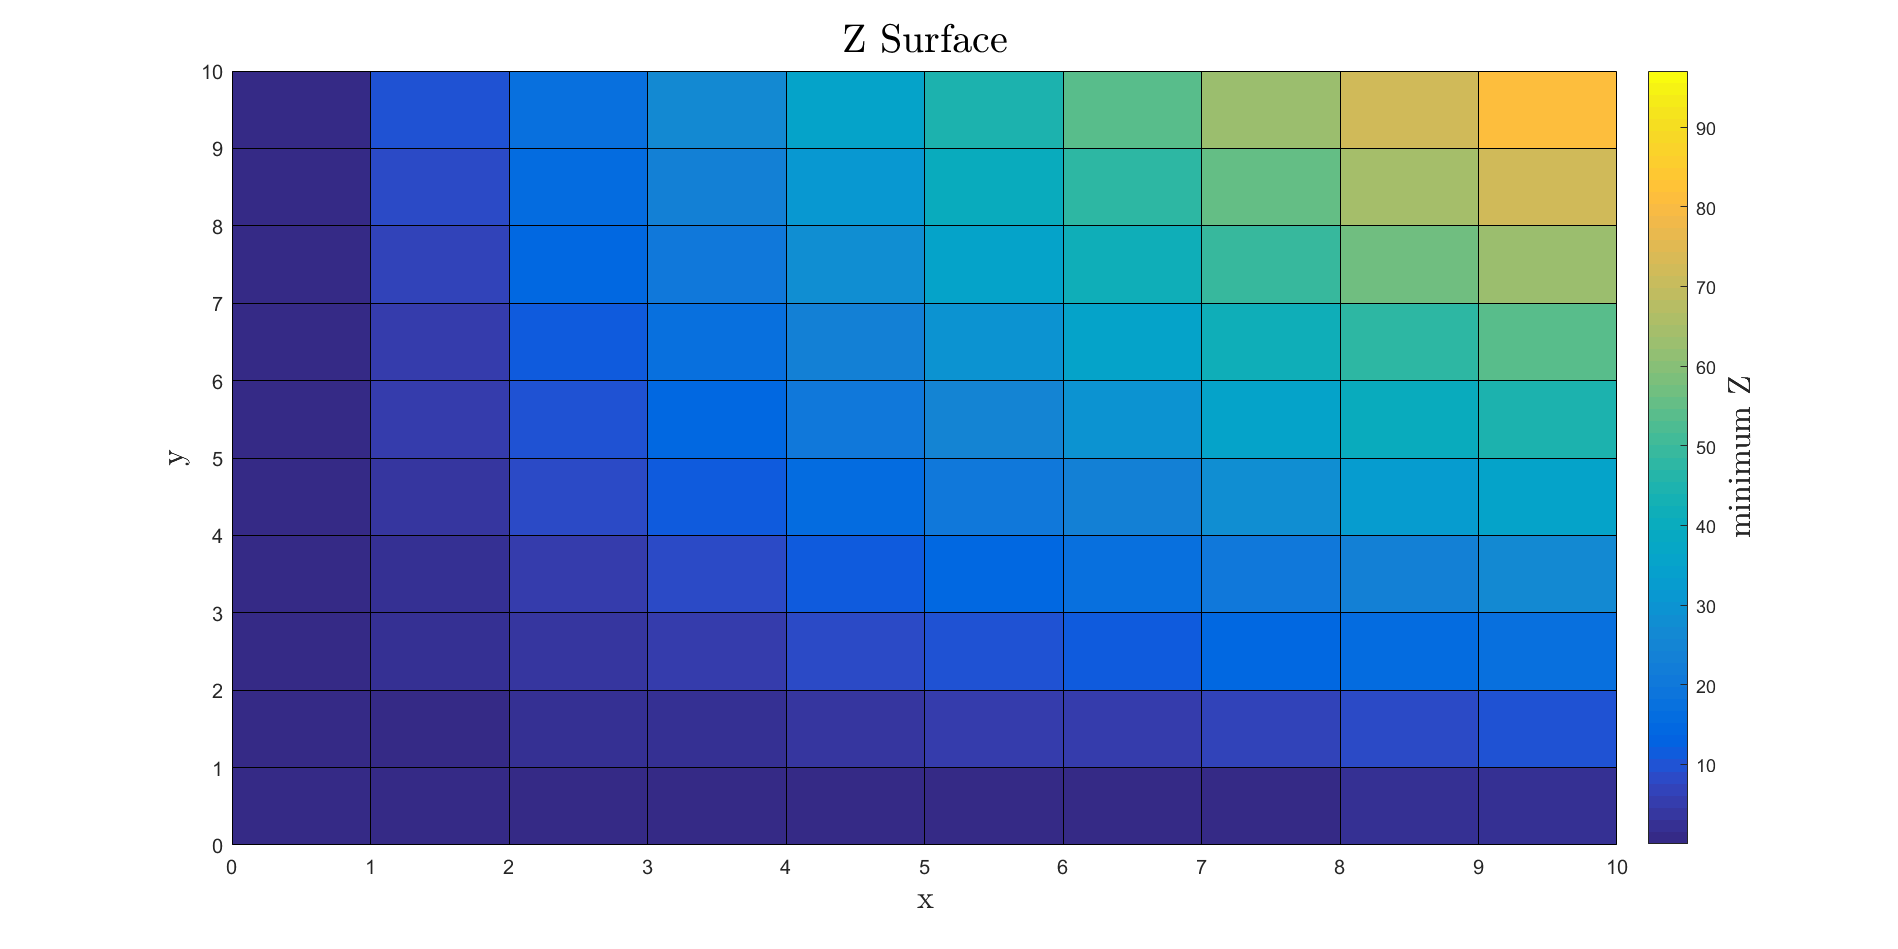
\includegraphics[width = \linewidth]{2d}
\end{figure}
\clearpage

\subsubsection*{Example IDW Voxels}
This example demonstrates generation of voxels.
\lstinputlisting[
label      = {alg:lsr},
style      = Matlab-editor,
basicstyle = \mlttfamily,
firstline  = 72,
lastline   = 81,
firstnumber= 72
]{../exampleIdw.m}

\begin{figure}[H]
	\centering
	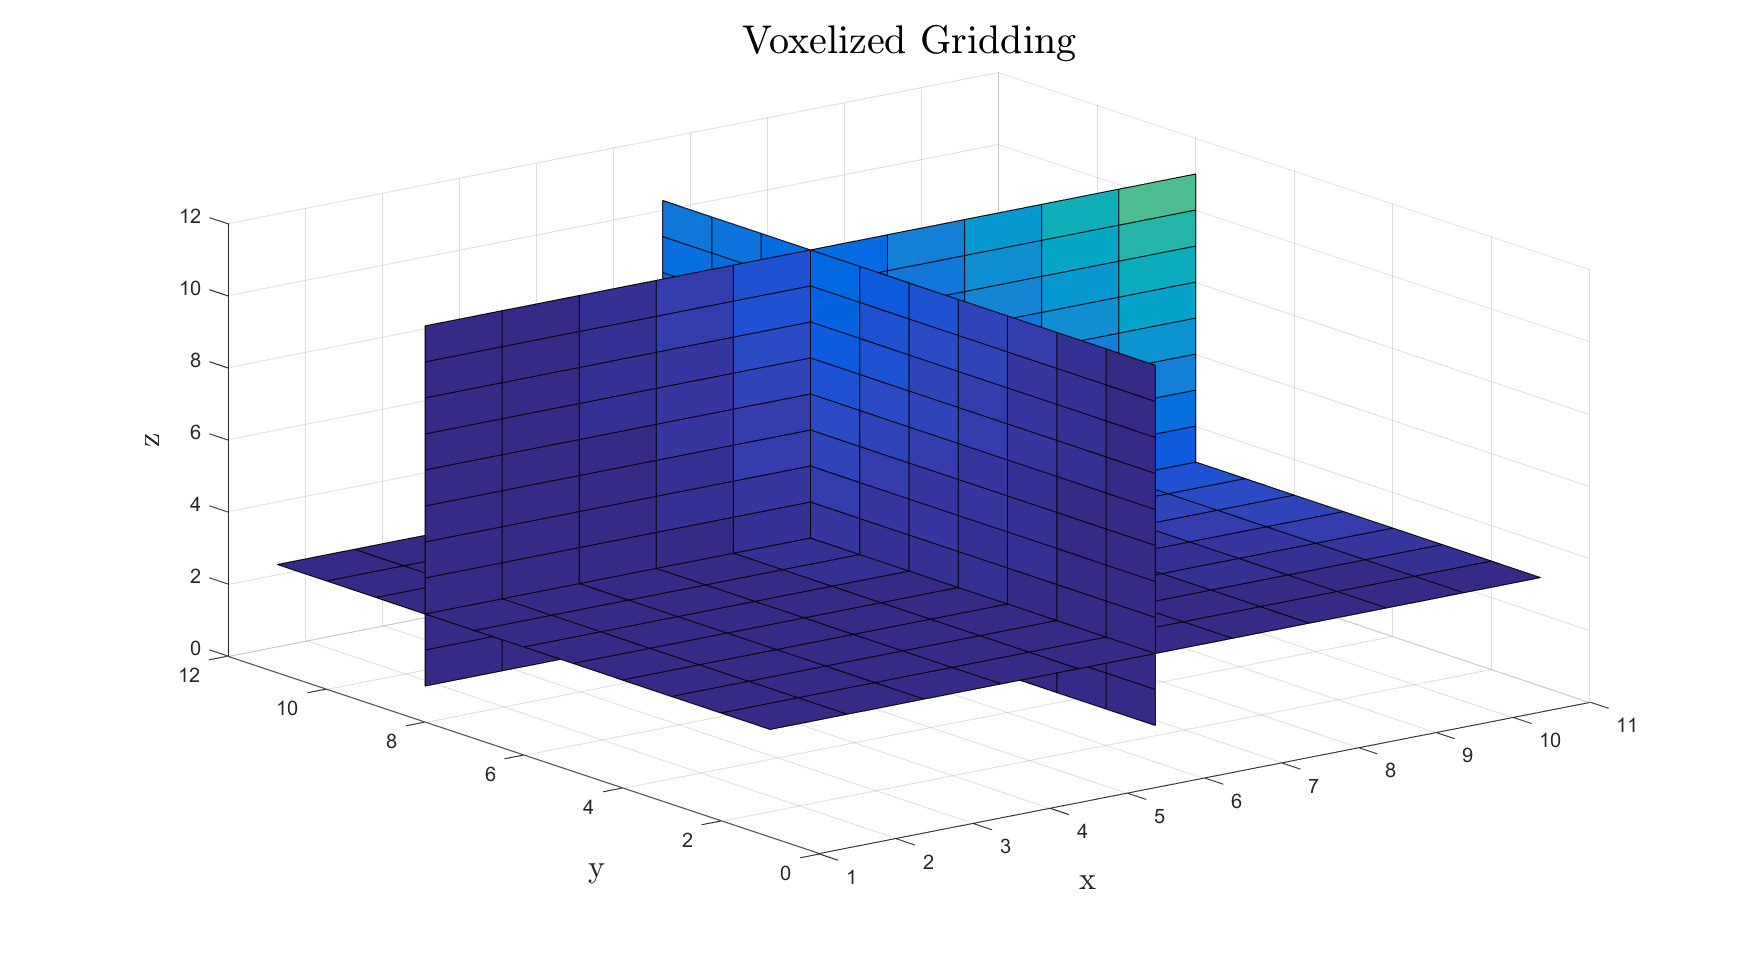
\includegraphics[width = \linewidth]{3d}
\end{figure}
\clearpage

\subsubsection*{Example Temporal Voxels}
This example demonstrates generation a 4d grid using x,y,z, and time.
\lstinputlisting[
label      = {alg:lsr},
style      = Matlab-editor,
basicstyle = \mlttfamily,
firstline  = 89,
lastline   = 95,
firstnumber= 89
]{../exampleIdw.m}

\begin{figure}[H]
	\centering
	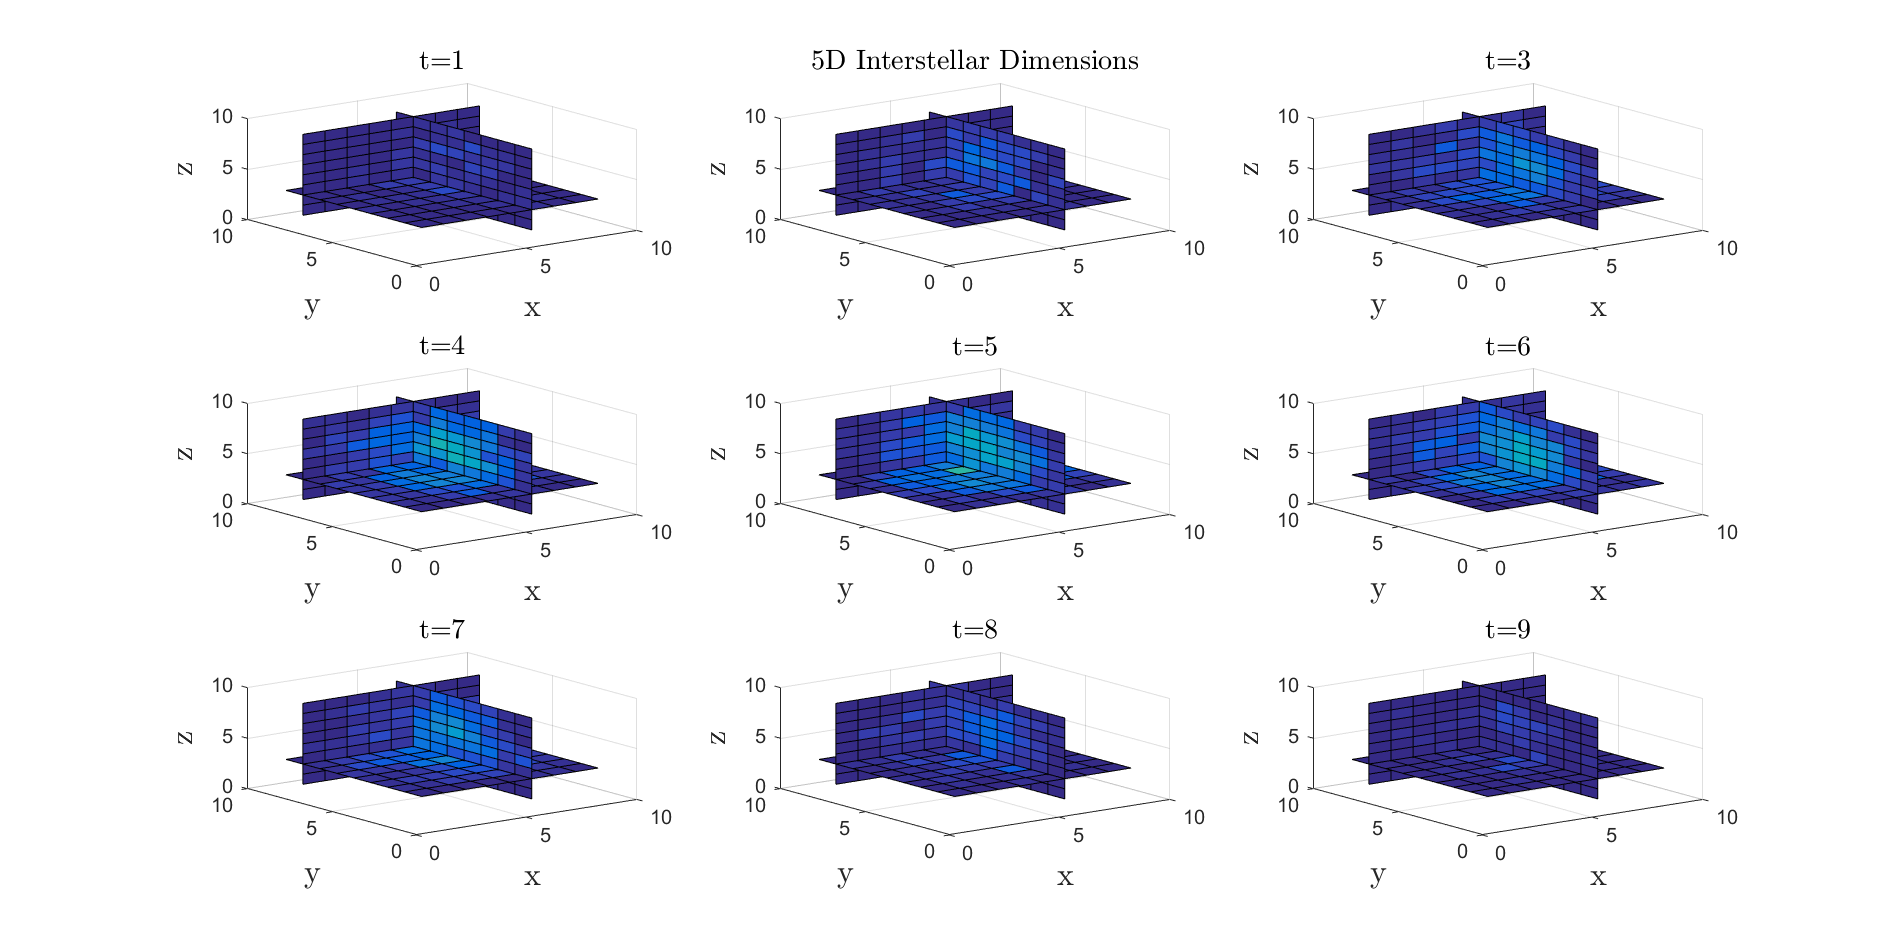
\includegraphics[width = \linewidth]{4d}
\end{figure}
\clearpage

\end{document}